%\noindent
\justifying
\setlength{\parskip}{1em}


In the field of document analysis, processing, and recognition, in the last two decades, several doucment image-to-image translation methods have been proposed. They usually aim at generating (automatically or semi-automatically) realistic document images, in terms of content (writings font, writings style, representations, etc.) and/or in terms of defects, noise, and distortions caused by the image acquisition procedure and scanning. \acp{GAN} are one of the most popular methods for image-to-image translation. They are effective for reducing divergence distance between the distribution of real data and the distribution of generated data. Several extended \ac{GAN} methods could be used to transform synthetic document images into realistic document images, such as DualGAN (Unsupervised Dual Learning for Image to Image Translation) \cite{yi2018dualgan}, DetectGAN \cite{Zhao.2020}, and \ac{MUNIT} \cite{huang2018multimodal}.

The DualGAN is designed for unsupervised image domain translation. It requires a minimal amount of annotation data and thus are suitable for the problem of document image-to-image translation. A DualGAN is similar method to \ac{CycleGAN}. DualGAN and \ac{CycleGAN} both aim for image domain translation without requiring paired training data to bridge the two image domains.




The \ac{MUNIT} 



The DetectGAN \cite{Zhao.2020}


\begin{figure}[!htbp]
        \begin{center}
    	\frame{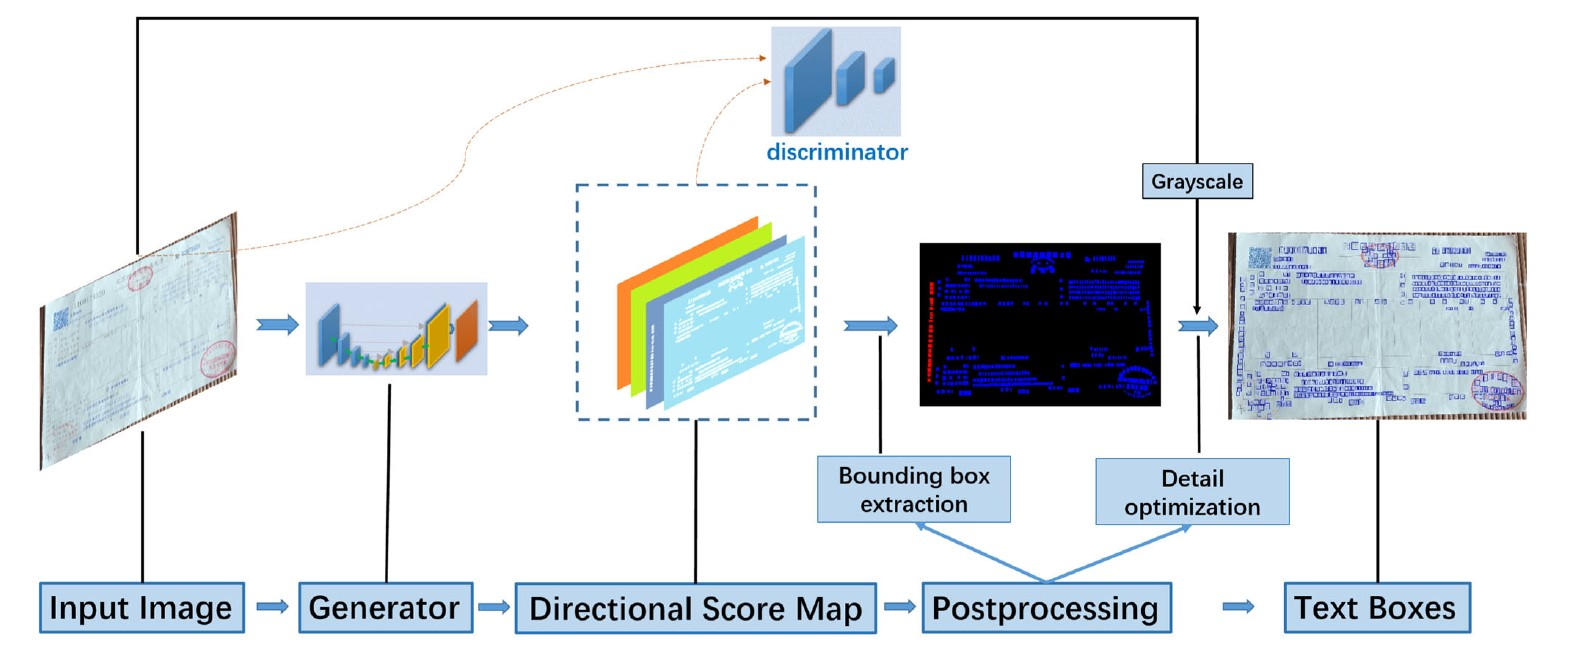
\includegraphics[scale=0.35]{images/DetectGAN.jpg}}
	    \caption[DetectGAN: GAN-based text detector for camera-captured document images.]{DetectGAN: GAN-based text detector for camera-captured document images \cite{Zhao.2020}.}
	    \label{fig:DetectGAN}
	    \end{center}
\end{figure}


Monika Sharma et al. \cite{sharma2019learning} proposed the solution for denoising and cleaning the document images using \ac{CycleGAN}. The denoising process using \ac{CycleGAN} can be visualized in the figure \ref{fig:LearningToClean}. But, this thesis strives to meet the noise distribution of real document images. The synthetic document images should be transformed into realistic document images. The opposite process of cited reference \cite{sharma2019learning}. However, Monika Sharma et al. affirmed a possibility of document image-to-image translation using \ac{CycleGAN}.

\begin{figure}[!htbp]
        \begin{center}
    	\frame{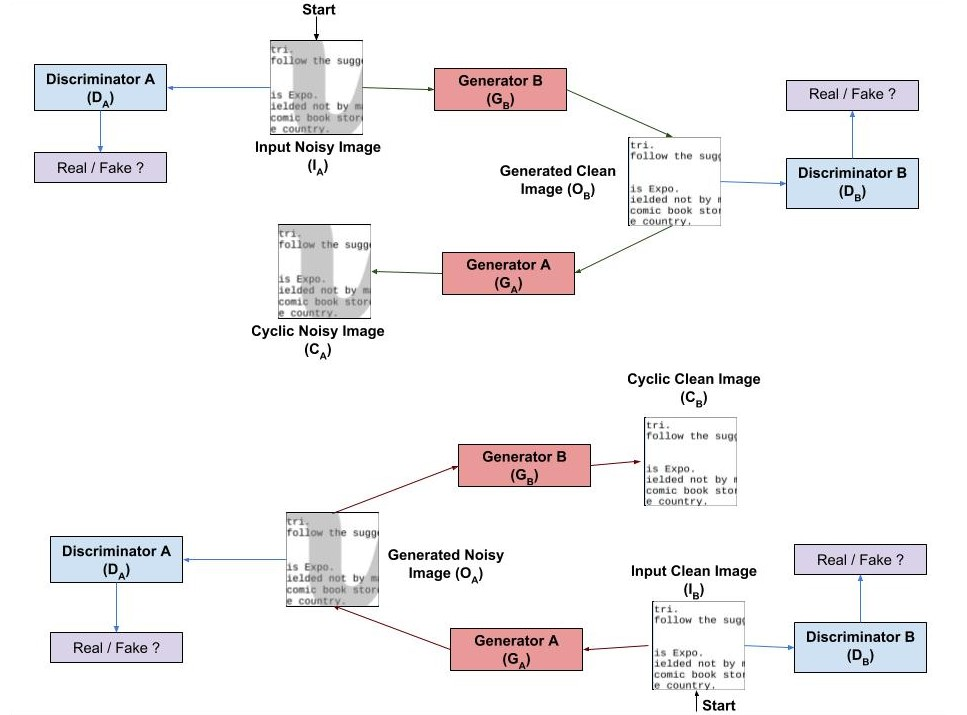
\includegraphics[scale=0.55]{images/LearningToClean.jpg}}
	    \caption[Overview of CycleGAN.]{Overview of \ac{CycleGAN} - It consists of two generators, $G_A$ and $G_B$ which map noisy images to clean images and clean to noisy images, respectively using cycle-consistency loss \cite{zhu2020unpaired}. It also contains two discriminators $D_A$ and $D_B$ which acts as adversary and rejects images generated by generators \cite{sharma2019learning}.}
	    \label{fig:LearningToClean}
	    \end{center}
\end{figure}




The above-mentioned evidence and literature survey are adequate to say \ac{CycleGAN} could be the prevailing approach to transform the synthetic document images into realistic document images. Ultimately, a large number of realistic document images are generated and the scarcity of labeled document images diminished. The deep learning models, \ac{OCR} systems, and \ac{HTR} systems can have a significant amount of data for training to produce highly accurate results.









































\begin{comment}

\acp{GAN} are one of the most popular methods for domain adaptation. \ac{GAN} was proposed by Ian J. Goodfellow et al. ~\cite{goodfellow2014generative} as an approach to generative modelling. The generative models are estimated via an adversarial process, in which simultaneously two models are trained, the generator model is trained to generate new samples, and the discriminator model tries to classify those samples as either real or fake. The two models are trained together in a minimax two-player game, adversarial, until the discriminator model is fooled about half the time, meaning the generator model is generating plausible samples. As the research in the field of generative modelling has increased numerous extended versions of \acp{GAN} are invented like \acp{cGAN} ~\cite{isola2018imagetoimage}, \acp{LSGAN} ~\cite{mao2017squares}, and \acp{CycleGAN} ~\cite{zhu2020unpaired}. These modified versions of \acp{GAN} are extensively used in the image-to-image translation techniques. For example, translation from horse image to zebra image and from apple image to orange image. 



As mentioned earlier the \acp{cGAN} are a general-purpose solution for mapping from the input image to the output image. This approach is effective at synthesizing photos from label maps \cite{cordts2016cityscapes}, reconstructing objects from edge maps \cite{article}, and colorizing images. The \acp{LSGAN} proposes to adopt the least squares loss function for the discriminator which resolves the vanishing gradient problem during the learning process. 

\end{comment}